\documentclass[a4paper,11pt]{article}
\usepackage[style=ieee,backend=bibtex]{biblatex} 
\usepackage{amsmath,amsfonts}
\usepackage{geometry}
\usepackage{bm}
\usepackage{longtable} % for 'longtable' environment
\usepackage{pdflscape} % for 'landscape' environment
\usepackage{rotating}
\usepackage{tabularx}
\usepackage{siunitx}
\usepackage{pgfgantt}
\usepackage{float}
\usepackage{svg}
\addbibresource{main.bib}

\DeclareSIUnit\feet{ft} % Yes I know feet aren't SI unit...
\DeclareSIUnit\year{y}


\ganttset{calendar week text={\small{\startday/\startmonth}}}

\begin{document}


\begin{titlepage}

% Center the content
\begin{center}

% Title
% \vspace*{3cm}
% ATTENTION: THIS IS A DRAFT VERSION. TODO: CHECK GRAMMAR AND PRESENTATION BEFORE SUBMITTING
{\LARGE\bfseries Evaluation of High-Powered Rockets as a CubeSat Qualification Platform} \\[3cm]



% Author's name
{\Large Author: Peter Tanner} \\[1cm]

% Supervisor's name
{\Large Supervisor: Dilusha Silva} \\[2cm] % \\[3cm]

% Degree text
{\large ATTENTION: THIS IS A DRAFT VERSION. TODO: CHECK GRAMMAR AND PRESENTATION BEFORE SUBMITTING}
{\large \textit{This thesis is presented in partial fulfilment of the requirements for the degree of Bachelor of Philosophy
(Honours) at the University of Western Australia}} \\[1cm]

% Faculty information
{\large Faculty of Engineering and Mathematical Sciences} \\[3cm]

{\large Word count: TODO:} \\
{\large Submitted: \today} \\[2cm]

\includesvg[width=0.5\textwidth]{images/UWA-logo-dark.svg} \\ 

\end{center}

\end{titlepage}
  
\newpage
\section{Abstract}

The CubeSat is a type of small satellite, initially conceived reduce the cost access to space to universities due to its small and standardised $\SI{10x10x10}{\centi\meter}$ cubic form factor. The total number of CubeSats launched into space is growing exponentially due to their low cost, doubling every $\SI{2.5}{\year}$, however the mission success rate has not increased significantly since 2018, levelling off at 75\% \cite{welle2020overview,bouwmeester2022improving}.

Vibration and shock tests are industry standard procedures which aim to emulate launch conditions, however they cannot perfectly replicate them \cite{gordon2015benefits}. Testing of CubeSats on suborbital high-powered rockets (HPR) is a novel qualification method that can potentially replicate launch conditions more accurately than traditional shaker table tests, and therefore better detect issues and improve the likelihood of mission success. While there have been tests of university CubeSats on high-powered rockets \cite{slongo2019pre}, there are no direct comparisons to shaker table tests to evaluate their effectiveness as a qualification method.

This paper outlines the construction of a data acquisition system to obtain acceleration data from the HPR launch, the HPR launch and vibration table tests and finally makes a direct comparison of the vibration environment on the HPR launch and vibration table.


\section{Acknowledgements}

I'd like to thank all the people and organisations who have supported me throughout this project. Dilusha Silva for being a wonderful mentor and for coordinating the project. Michal Zawierta for his expertise flying drones for the drone tests of the CubeSat. Jamir Khan for being a wonderful friend and engineer who worked on the mechanical side of this project, including construction of the high-powered rocket, and for putting up with all my delays. Timothy Ludovico for designing the camera payload and being all around wonderful to work with. Jeremy Marelich and AVI for providing their shaker table facilities and conducting the tests. UWA Aerospace for being a wonderful institution who has been with me from first year through my growth as an engineer and has supported me through this project. Space Angel for creating this project and providing expertise and connections to the Indian Institute of Space Science and Technology (IIST). International Space Centre for supporting this project with funding.


\newpage
\tableofcontents
\newpage

% TODO: FOR MEETING
% WHAT WOULD THIS THESIS BE ASSESSED UNDER?
% IS THERE A LATEX TEMPLATE USED BY MRG?
% I AM WORRIED THIS PROJECT WILL BE ASSESSED TOO MUCH WITH RESULTS AND DISCUSSION WHEN A LOT OF MY CONTENT IS ON THE EXPERIMENTAL DESIGN , IS THIS AN ISSUE?

% CRITERIA:
% 10% SCOPE
% PROJECT BODY (ASSUME EXPERIMENTAL PROJECT):
%   20% INTRODUCTION AND LITERATURE REVIEW
%   15% EXPERIMENTAL DESIGN
%   35% RESULTS AND DISCUSSION
% 10% CONCLUSION AND FUTURE WORK
% 10% PRESENTATION (SHOULD BE GUARANTEED...)

% USING FORMULA $SECTION/80%
% INTRODUCTION AND LITERATURE REVIEW: 3000 TO 4500 WORDS
% EXPERIMENTAL DESIGN: 2250 TO 3375
% RESULTS AND DISCUSSION: 5250 TO 7875
% CONCLUSION AND FUTURE WORK: 1500 TO 2250

\renewcommand{\listfigurename}{
  \section{List of figures}
}
\listoffigures
\cleardoublepage
\renewcommand{\listtablename}{
  \section{List of tables}
}
\listoftables
\cleardoublepage

\section{Introduction}
\subsection{Background}
% Introduction or Background This provides the reader with the context of the project. For example, what is the application area, why is it important, what (in general terms) has been done before?
The University of Western Australia (UWA) Microelectronics Research Group (MRG) is developing a CubeSat with a camera system to obtain plant information. The CubeSat is a type of small satellite, initially conceived reduce the cost access to space to universities due to its small and standardised $\SI{10x10x10}{\centi\meter}$ cube form factor. The total number of CubeSats launched into space is growing exponentially due to their low cost, doubling every $\SI{2.5}{\year}$, however the mission success rate has not increased significantly since 2018, levelling off at 75\% \cite{welle2020overview,bouwmeester2022improving}. For most single-launch satellites, increased testing is the optimal strategy to minimise failure \cite{bouwmeester2022improving}.

Common CubeSat qualification tests include vibration, shock and thermal vacuum testing \cite{welle2020overview} which are intended to replicate the conditions of launch and space. Vibration and shock tests are an industry standard procedure, however they do not perfectly replicate the conditions at launch \cite{gordon2015benefits}. Testing of CubeSats on suborbital high-powered rockets (HPR) is a novel qualification method that can potentially replicate launch conditions more accurately than established shaker table tests, and therefore better detect issues and improve the likelihood of mission success. This qualification method has only been used on the FloripaSat-I CubeSat on a higher performance suborbital sounding rocket, to complement common qualification tests. MRG will be using standard qualification tests and HPR testing as part of the qualification phase.

\subsection{Problem identification}
% Problem Identification What is the problem that you are trying to solve, or the hypothesis that you are intending 
% to test? What is your intended contribution to the state of the art?
Current shock and vibration tests do not perfectly replicate conditions at launch \cite{gordon2015benefits,nath2022study}, which could be one of the factors for high CubeSat mission failure rates. A potential improvement is the use of a high-powered rocket to more accurately emulate launch, which can therefore decrease mission failure rates. However, there are no comparisons between existing shaker table methods and high-powered rocket qualification to properly evaluate whether it will be an improvement over the standard tests.

\subsection{Intended contribution}
% Problem Identification What is the problem that you are trying to solve, or the hypothesis that you are intending to test? What is your intended contribution to the state of the art?

This research will achieve two goals. Firstly, it will develop a platform for testing CubeSats on HPRs to identify practical design considerations and issues when developing for HPRs. Secondly, the platform will be also used to measure acceleration data on various parts of the CubeSat during standard testing and during the HPR flight, which will be used to evaluate the effectiveness of the HPR qualification method compared to standard shaker table tests.

% The research will determine if a high-powered rocket is a more accurate representation of the vibration conditions a CubeSat will experience during launch compared to a traditional single-axis vibration and shock testing method.

% TODO: GOAL: 3000 words :((

% This project will design and manufacture a system which provides power and communications to a CubeSat and provides sensors such as accelerometers, temperature and humidity sensors which are required for testing. The system should have the same communication interfaces and power capabilities which the POEM launch platform can provide to a single CubeSat, and should be constructed in a way that it is functionally identical to the POEM launch platform.

\section{Literature Review}
% Literature Review or Previous Work Explain the literature (e.g. refereed research papers) or previous body of work (e.g. previous projects within the research group) on which your investigation is based. This should not simply be a linear account, but rather a synthesis of what is important from what has gone before. It will often be a hierarchical account, moving from a general understanding of the field, to identification and expansion of work that is specifically relevant to your project

This literature review will cover the current testing methods used in CubeSats, the use of suborbital rockets as a qualification method and cover the types of sensors and systems required to record these tests.

\subsection{Standard satellite qualification methods}
Satellites undergo a panel of qualification tests to maximise the chance of mission success, and may be required by the launch provider to demonstrate that there is minimal risk of the satellite to the launch vehicle and other payloads which may be present. There are multiple satellite qualification standards, an example is the NASA General Environmental Verification Specification (GEVS) which is a panel of tests including electromagnetic compatibility (EMC), thermal, acoustic and vibration tests that are required for all NASA Goddard Space Flight Center projects \cite{nasa-gevs}. Other standards include ISO-15864, JERG-2-002, NASA-STD-7002A, ECSS-E-ST-10-03C and SMC-S-01 \cite{cho2012overview}. While these standards have flight heritage, being used on many successful payloads, they were designed for medium or large satellites, and therefore fully complying with these standards are out of the budget of most university CubeSat programs \cite{cho2012overview}. While is no widely used test standard for CubeSats currently in use, since most CubeSat projects perform the minimum panel of tests required by the launch provider to minimise cost, there is a de facto minimum series of tests which are random vibration, shock and thermal vacuum testing \cite{welle2020overview}.

% \subsection{Thermal vacuum}
% Thermal vacuum tests replicate the thermal conditions of space to verify a satellite's operation under these conditions and to check for workmanship issues \cite{brown_elements_2002}.

% A thermal vacuum bakeout creates high temperature, high vacuum conditions which promote outgassing \cite{jiao2019outgassing} - the outgassing products are collected and analysed to ensure it does not damage any payloads or the launch vehicle \cite{nasa-gevs}.

% A thermal vacuum cycle test involves periodically cycling the temperature between low and high to replicate the temperature swings experienced by the satellite as it orbits between the day and night sides \cite{nasa-gevs}. Temperatures may range start between $\SI{-40}{\celsius}$ \cite{bulut2021thermal} and $\SI{-30}{\celsius}$ \cite{mason2018cubesat} and range to up to $\SI{60}{\celsius}$ \cite{mason2018cubesat} to $\SI{80}{\celsius}$ \cite{bulut2021thermal}.

% A thermal vacuum balance test assesses the satellite's thermal performance in thermal equilibrium, in both hot and cold cases \cite{nasa-gevs} and is used to validate the thermal model \cite{bulut2021thermal}.

% % Thermal vacuum tests are routinely performed 

% \begin{figure}[H]
%   \centering
%   \includegraphics[width=0.75\textwidth]{images/temperature.png}
%   \caption{Thermal model of a satellite \cite{bulut2021thermal}}
% \end{figure}

% % TODO: write more shit

\subsection{Vibration}
Vibrations are experienced by satellites during transportation and loading, and most prominently during launch \cite{brown_elements_2002}. The purpose of vibration testing is to ensure that the satellite will survive transportation and launch conditions, and to find workmanship errors \cite{brown_elements_2002,gordon2015benefits}.

\subsubsection{Random vibration / sine sweep vibration test}
In the random vibration test, a uniform vibration spectrum is applied to the satellite which tests all the resonant frequencies of the satellite \cite{nieto2019cubesat}. This range includes frequencies on the magnitude of $\SI{100}{\hertz}$, since higher frequencies couple to the satellite through acoustic means rather than through the structure \cite{gordon2015benefits}. A sine sweep vibration test is similar, but instead of the frequency being randomly sampled it is swept through sequentially from either low to high frequency or vice versa. An example of a random vibration test is shown in figure \ref{fig:random}, where frequencies up to $\SI{100}{\hertz}$ were evaluated, and higher frequencies above $\SI{100}{\hertz}$ were attenuated proportional to frequency.

\begin{figure}[H]
  \centering
  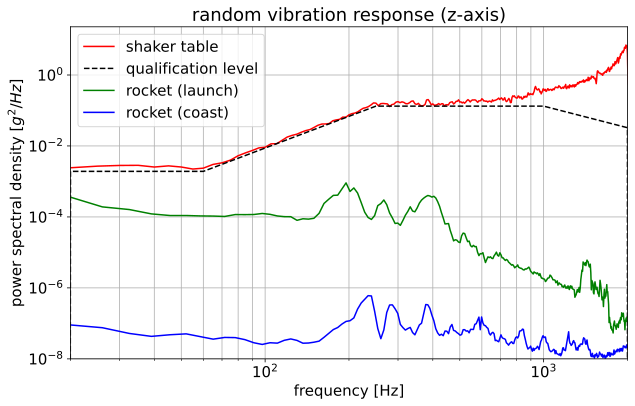
\includegraphics[width=0.75\textwidth]{images/random.png}
  \caption{Random vibration test \cite{nieto2019cubesat}}
  \label{fig:random}
\end{figure}

The limitations of random vibration tests is that the shaker and table will have different modes than the launch vehicle and payload mount, resulting in the test response not perfectly matching the flight response \cite{gordon2015benefits,aglietti2019spacecraft}. Gordon and Kern argue that this difference is not a factor in practice since shaker tests are "not intended to be a strength test"  \cite[p.~7]{gordon2015benefits} and that components "should have been strength qualified prior to integration" \cite[p.~7]{gordon2015benefits}. Component level is argued as a best practice in the CubeSat community \cite{rawsonbest}, however some argue that component level testing is not suited to the short timeline of university CubeSat projects and that more effort should be put into integration testing \cite{decker2016systems}. If a testing program focuses on integration testing, then this mismatch between shaker table and flight response could result in the CubeSat not being properly qualified.

Finally, although 6 degrees of freedom (DOF) vibration tables exist which can replicate the vibrations experienced in all dimensions during launch, most satellites are still tested with single-axis or random input shakers which only provide one dimension \cite{gordon2015benefits,aglietti2019spacecraft,nath2022study}. While Gordon and Kern \cite{gordon2015benefits} state that these limitations are adequately managed by testing in all three orthogonal axes separately, Aglietti and Nath \cite{nath2022study} created a model of three, two and single axis vibration tests and found that to match the 3 DOF response with a single DOF table, the satellite needed to be subjected to 2.5 times the $g_\text{rms}$ forces than in 3 DOF testing, leading to the satellite being over designed \cite{nath2022study}.




\subsubsection{Quasi-static acceleration test (QAT)}
A quasi-static test replicates the liftoff stage of flight, where there is a combination of random vibration from engines and quasi-static axial acceleration from the engine and other external forces on the launch vehicle \cite{nieto2019cubesat,brown_elements_2002}, which are approximated as constant forces at selected frequencies as shown in figure \ref{fig:qatforces}. The QAT is usually compared to results from coupled loads analysis, where all forces are assumed to be applied to the satellite through the launch vehicle as shown in figure \ref{fig:cla} \cite{dickens2001coupled}.

\begin{figure}[H]
  \centering
  \includegraphics[width=0.75\textwidth]{images/qat.png}
  \caption{Quasi-static acceleration test. The input profile high acceleration from $\SI{20}{\hertz}$ to $\SI{21}{\hertz}$, resulting in the response having a force of 10.8 \textit{g} acceleration around this frequency \cite{nieto2019cubesat}}
  \label{fig:qatforces}
\end{figure}

\begin{figure}[H]
  \centering
  \includegraphics[width=0.3\textwidth]{images/cla.png}
  \caption{Coupled loads model \cite{dickens2001coupled}}
  \label{fig:cla}
\end{figure}

The first limitation of a quasi-static acceleration test is that the shaker table cannot apply the peak response evenly on the CubeSat that is predicted by coupled loads analysis (CLA) \cite{gordon2015benefits}. Again, Gordon and Kern state that these limitations are addressed by component-level strength qualification. They also state that applying the peak response evenly is not necessary, since if an item does not fail, the correctly applying the response evenly does not greatly increase its likelihood of failing \cite{gordon2015benefits}.
The second limitation is there is a difference in modes, since a quasi-static acceleration test also contains random vibrations \cite{gordon2015benefits}.



\subsection{Vibroacoustic testing}

As stated, low frequency vibrations from $\SI{0}{\hertz}$ to $\SI{100}{\hertz}$ tend to couple well through the payload mount, however high frequency vibrations above $\SI{100}{\hertz}$ are more efficiently imparted on the satellite acoustically \cite{gordon2015benefits}. These acoustic loads have an effect on payload electronics \cite{casalino2012rocket}, and primarily originate from the highly turbulent engine exhaust \cite{casalino2012rocket}.

Vibroacoustic testing is not necessary for CubeSats due to their small surface area \cite{nasa-gevs}, since the magnitude of the acoustic response is proportional to the satellite's surface area to mass ratio \cite{brown_elements_2002}, therefore the effect of the acoustic loads is negligible. Instead, vibroacoustic testing is more relevant for large and light payloads such as solar panel arrays \cite{brown_elements_2002}, therefore it will not be part of this research.

\subsection{Shock}

Shock is experienced by satellites when pyrotechnics are detonated or deflagrated during events such as staging and ignition, the response appears as a range of decaying sinusoids in the $\SI{100}{\hertz}$ to $\SI{10}{\kilo\hertz}$ frequency range \cite{brown_elements_2002}, which decay in $\SI{5}{\milli\second}$ to $\SI{15}{\milli\second}$ \cite{brown_elements_2002}. The spectrum extends up to $\SI{40}{\kilo\hertz}$, however for analysis frequencies above $\SI{10}{\kilo\hertz}$ are assumed to be non-damaging \cite{bement1995manual,nasa-pyroshock}. Pyroshock may cause peak accelerations of up to 10000 \textit{g} \cite{nasa-pyroshock}. High explosives are primarily used for explosive elements on rockets in combination with some low explosives for initiators \cite{bement1995manual}.

Shock is tested using a shock-generating device which is applied to the satellite along all three axes \cite{nasa-gevs,nasa-pyroshock}, the shock generating device for a CubeSat can be an electrodynamic shaker table \cite{nieto2019cubesat} with a half-sine, pulse profile \cite{nieto2019cubesat}. The shock test has similar limitations as the random vibration test, since it also uses a vibration table to affect the satellite.

Shock tests are compared using the shock response spectrum (SRS), which plots the maximum acceleration per frequency bin. The SRS contains an octave slope which rises to the first resonant frequency called the "knee frequency". The octave slope can be approximately 9 dB/octave to 12 dB/octave depending on distance to the source.

\begin{figure}[H]
  \includegraphics[width=0.5\textwidth]{images/pyroshock2.png}
  \includegraphics[width=0.5\textwidth]{images/pyroshock1.png}
  \caption{Shock response spectrum of and time-domain shock response. Left: near-field (close to shock source). Right: far-field (distant from shock source) \cite{nasa-pyroshock}}
  \label{fig:pyroshock}
\end{figure}


\subsection{Rocket testing of CubeSats}
\subsubsection{Sounding rockets}
Sounding rockets are a class of suborbital rocket used between $\SI{40}{\kilo\meter}$ and $\SI{200}{\kilo\meter}$, above where weather balloons operate \cite{seibert2006history}. While sounding rockets have been used to launch many CubeSats as the primary launch vehicle for suborbital CubeSat missions, such as in the REXUS-25 mission \cite{pont2019rexus}, there has been only one published instance of sounding rockets being used as an additional qualification platform for a CubeSat \cite{slongo2019pre}. The FloripaSat-I CubeSat was tested on a VSB-30 sounding rocket \cite{slongo2019pre} to qualify the CubeSat under launch conditions. This qualification method was intended not to replace, but to complement standard vibration and shock qualification methods \cite{slongo2019pre}. The test measured these launch conditions through the MPU6050 6 DOF inertial measurement unit (IMU) \cite{slongo2019pre}.

\begin{figure}[H]
  \includegraphics[width=0.5\textwidth]{images/floripa-accel.png}
  \includegraphics[width=0.5\textwidth]{images/floripa-rot.png}
  \caption{Acceleration in time domain (Left), Angular velocity in time domain (Right) during the launch of FloripaSat-I \cite{9316404}}
  \label{fig:accel-rot}
\end{figure}

While this study does show the time-domain accelerometer and gyroscope measurements from the sounding rocket launch in figure \ref{fig:accel-rot}, it does not compare the data to other qualification tests in the FloripaSat-I campaign, such as traditional vibration and shock testing. Additionally, the launch data was not presented in the frequency domain through the boost and coast phases of the flight, meaning they could not be compared to the acceleration spectra which was shown for the shaker table testing in figure \ref{fig:shaker}.

\begin{figure}[H]
  \includegraphics[width=0.5\textwidth]{images/floripa-random-spectrum.png}
  \includegraphics[width=0.5\textwidth]{images/floripa-sinusoid.png}
  \label{fig:shaker}
  \caption{Random vibration (Left) and sine sweep (Right) tests on a shaker table during the qualification of FloripaSat-I \cite{9316404}}
\end{figure}

Another shortcoming of the study is that a shock test using a half-sine pulse was not performed. The use of a sounding rocket is a potential method of qualifying the CubeSat's ability to tolerate shocks since there will be shock events when pyrotechnics are lit to stage the rocket, although the forces will have intensity than on a larger launch vehicle.

\subsubsection{High-powered rockets (HPR)}
While sounding rockets have a significantly lower cost compared to an orbital-class launch vehicle, they cost \$1 million USD per launch to launch $\SI{200}{\kilo\gram}$ on average \cite{jurist2009commercial}, resulting in a specific cost of \$5000 USD/kg, which is still a large amount for university CubeSat programs. High-powered rockets (HPR) are a lower-performance but cheaper alternative to sounding rockets, which can leverage the design expertise of university rocketry teams while having similar qualification potential as sounding rockets. A single stage level 3 certification rocket can reach altitudes above $\SI{10000}{\feet}$ \cite{canepa2005modern} for a cost of only \$1200 USD \cite{canepa2005modern}. Despite the potential cost benefits, there have not been any published instances of a HPR being used to qualify a CubeSat.

One potential issue with HPRs as a qualification platform for shock is that low explosive black powder is used \cite{canepa2005modern} which has different explosive characteristics, such as a subsonic flame front, compared to the high-explosives used in launch vehicles \cite{bement1995manual} and will therefore produce different shock responses. One study \cite{wang2023numerical} performed finite element analysis of igniters filled with low explosives including aluminium potassium perchlorate and boron potassium nitrate and determined the SRS, shown in figure \ref{fig:lowsrs}. Compared to the SRS of high-explosives in figure \ref{fig:pyroshock}, where at a frequency of 1 kHz the acceleration is over $10^2$ \textit{g} \cite{nasa-pyroshock}, in these low explosive simulations the acceleration at 1 kHz is only $10^1$ \textit{g} \cite{wang2023numerical}. Therefore, it is hypothesised that HPRs will not be useful for shock qualification since the response of low explosives is different from the high explosives used on launch vehicles.


\begin{figure}[H]
  \centering
  \includegraphics[width=0.75\textwidth]{images/deflagration.png}
  \caption{Shock response spectrum from computer modelling of an igniter based on the low explosive aluminium potassium perchlorate \cite{wang2023numerical}}
  \label{fig:lowsrs}
\end{figure}

;
% \section{Methodology};
% % Methodology How you plan to solve the problem or resolve the hypothesis.;
;
% The methodology will consist of two phases:;
;
% \begin{enumerate};
%   \item Development and construction of a low-cost POEM emulation system and sensors to measure the vibration and shock on the CubeSat during the HPR launch and shaker table tests, and to ensure recovery of the HPR and CubeSat.;
%   \item Comparison of the recorded data from the HPR launch and shaker table tests against the parameters given by the launch provider.;
% \end{enumerate};
;
\section{First revision of test and POEM emulation electronics}

The POEM provides services such as tracking, telemetry and command (TT\&C), electrical power system (EPS) and on-board data handling (OBDH) to the CubeSat, therefore these systems are not integrated into the CubeSat under test and must be provided by a separate system on the HPR which emulates the POEM services. The POEM emulator consists of three PCBs: A combined EPS and OBDH board, a tracking board and a telemetry and command board.

\subsection{On-board data handling (OBDH)}
Two OBDHs are arranged in a dual redundant configuration and are linked to each other via controller area network (CAN) bus. When the hot spare detects that the primary OBDH is outputting bad data or is not responding, the secondary OBDH will take over control of the communications link. This redundancy ensures the likelihood of not obtaining experiment data for this research is minimised. In the best case, this will provide two independent data sources for research. Both OBDHs will still store data to their respective eMMC modules for post-flight analysis.

\subsection{Accelerometers}
MEMS accelerometers, which will provide the data for this analysis, are located on independent modules and on the OBDH computer. The low-cost LSM6DSO accelerometer will be used due to its low cost and acceleration range of 16-\textit{g} and bandwidth of up to $\SI{6664}{\hertz}$ \cite{lsm6dso-datasheet}, which will be used to cover the quasi-static acceleration and random vibration cases. As shown in figures \ref{fig:random} and \ref{fig:qatforces}, the \textit{g}-levels and bandwidth are relatively low and are met by the LSM6DSO.

The independent accelerometer modules will contain a microcontroller, regulator and accelerometer in a small package which can be mounted at various points on the CubeSat, to measure how evenly the response is applied to the CubeSat. The microcontroller will compress the accelerometer data and send it to the OBDH over CAN bus. The OBDH will generate a clock synchronisation signal to ensure the accelerometer measurements are synchronised. The modules will be attached to the CubeSat using adhesives due to its acceptable performance at the frequencies being measured, and ease of use compared to screws.

Measuring the shock response is significantly more difficult due to the high acceleration levels and the large bandwidth \cite{nasa-pyroshock}, which are not well-suited for low-cost MEMS accelerometers. Instead of measuring the full spectrum, the slope will be measured and compared using the low-cost ADXL373 accelerometer which can measure up to 400-\textit{g} at 2.56 kHz, which is enough to characterise the slope, which is the only parameter required to show that a rocket is inadequate for qualifying shock.

% TODO: shock response

\subsection{Electrical power system (EPS)}
A 2S lithium-ion battery pack and two 5V boost converters will be used to power CubeSat and the emulator. Two independent EPS will be connected in an OR-ing configuration so that if one fails, the other will provide power. The CubeSat and emulator will have separate boost converters, and the power to the CubeSat is capable of delivering the full 5V @ 3A which is the specified amount of power available to the CubeSat on the POEM.

\subsection{Telemetry and command}
An RFD900x radio will be used to downlink the data from the CubeSat and the engineering sensors. This link is optimised for relatively high speed and to have the full 300 kbps capacity that the POEM can provide to the CubeSat. The experiment data required for this research will be downlinked as part of the engineering data, to ensure that data is available to continue research in case the rocket crashes and the onboard memory is destroyed.

The tracking and command system will be on a separate low-bandwidth LoRa radio which is optimised for high link budget and reliability.


\subsection{GNSS Tracking}

The GNSS tracking board contains a standard precision NEO-M9N GNSS receiver and the ZED-F9P differential GNSS (DGNSS) receiver. A NEO-M9N was selected against other standard GNSS receivers due to its high maximum position, velocity and time (PVT) update rate of $\SI{25}{\hertz}$. The main purpose of the NEO-M9N is to serve as a simple backup GNSS receiver for reliable tracking purposes, since it does not require an RTK data stream.

The ZED-F9P differential receiver has centimetre-level accuracy and will enable the heading of the rocket to be accurately determined, which is required for this research since the heading may change throughout the flight and this will need to be accounted for when analysing the data since there are 6 DOF, instead of just one in traditional shaker table tests.

\section{Second revision of test and POEM emulation electronics}
\subsection{On-board data handling (OBDH)}
\subsection{Accelerometers}
\subsection{Electrical power system (EPS)}
\subsection{Telemetry and command}
\subsection{GNSS Tracking}


\section{Vibration table testing}
\subsection{UWA vibration table test setup}
\subsection{AVI vibration table test setup}

\section{Rocket tests}
\subsection{First test with H motor}
\subsection{Second test with K motor}

\section{Drone tests}
\subsection{First test}
\subsection{Second test}

% TODO: QUESTIONS - SHOULD I INCLUDE FREEZER/THERMAL TESTING?
% TODO: seems like a lot of honors thesis go into way more detail in the headings, what's up with that
% TODO: is it better to discuss each system as a whole or break it up into subsystems and show the differences as shown above
% TODO: I am worried this paper will have too much design and not enough data.
% TODO: How should i include code I used to write data? I noticed other papers broke it off into an algorithms section displaying pseudocode, does it have to be pseudocode?
% TODO: Is the abstract for the seminar and the thesis the same (in terms of length/content)?

\section{Data collection and analysis}

The system will be used for the vibration tests on a shaker table, and the rocket test. The data will be recorded as a time series on the OBDH memory. The time series data will be transformed into the frequency domain since existing studies have presented frequency domain plots to present and analyse the response of the system to a test \cite{nasa-pyroshock,nieto2019cubesat}. For the rocket test, the analysis will be split over the several phases of flight - launch, thrust, coast and parachute deployment events, since the forces involved are different in all of these phases.

\subsection{Shock}
\subsubsection{Vibration table results}
\subsubsection{HPR results}
\subsubsection{Comparison of methods}
In the launch and parachute deployments, where pyrotechnics are ignited, an analysis of the shock response spectrum will be performed. This will involve creating the shock response spectrum for the rocket test and shaker table tests, then comparing the slope up to ~1 kHz. If the rocket test SRS slope is on the same order of magnitude as the gradient found in \cite{wang2023numerical} for other low explosives, and it is less than the slope of the SRS from the shaker table tests, then this will show that rocket testing is not an adequate qualification method for shock.

\subsection{Random}
\subsubsection{Vibration table results}
\subsubsection{HPR results}
\subsubsection{Comparison of methods}
The coast phase, where the rocket motor has burnt out but is still approaching apogee, will be compared to the random vibration test. The random response spectrum will be compared to the spectrum of the rocket test to check how uniformly distributed the rocket test is.

\subsection{Quasi-static acceleration}
\subsubsection{Vibration table results}
\subsubsection{HPR results}
\subsubsection{Comparison of methods}
The boost phase will be compared to the quasi-static acceleration tests on the shaker table. It is expected that the acceleration force on the HPR will be greater than those experienced on the launch vehicle, however the key characteristic - a peak in acceleration over a narrow frequency band - should be the same.

\section{Conclusion}
\subsection{Future work}

\section{References}

\printbibliography[heading=none]

\section{Appendix}



\end{document}
